\chapter{Implementation}\label{ch:impl}

This chapter focusses on the practical side and on the internal workings of the system we developed.
It explains the steps from receiving the input program to outputting a list of anomalies which hint at potentially missing method calls.
We give details about design decisions taken and the reasoning behind them, pitfalls that had to be overcome and the trade-offs that had to be accepted.
Additionally, we explore some of the mistakes made and dead ends that we encountered.

\section{Overview}

Our system is (primarily) a system that detects missing method calls.
It works by statically analyzing a given software application, extracting the type usages it contains and finally determining if any of them are anomalous by the majority rule as described in Chapter~\ref{ch:dmmc}.
The end result is a list of locations which are potentially missing a method call.
Given a software system which shall be tested for anomalies, the following steps have to be realized:

\begin{enumerate}
    \item Extract all type usages from the software;
    \item For each type usage $x$, among them:
    \begin{enumerate}
        \item Search for type usages which are exactly similar to $x$ (i.e.\ calculate $E(x)$);
        \item Search for type usages which are almost similar to $x$ (that is determine $A(x)$);
        \item Calculate the strangeness score of $x$;
        \item Extract the list of potentially missing calls and their likelihood $\phi$;
    \end{enumerate}
    \item Output a list of anomalous type usages, sorted by their $\operatorname{S-score}$s, together with the calls they are potentially missing.
\end{enumerate}

\begin{figure}[h]
\centering
\begin{tikzpicture}
    \tikzset{vertex/.style={draw,rounded corners,align=center}}
    \tikzset{edge/.style = {->,> = latex'}}

    % start dot
    \node[fill=white] (startTxt) {Application};
    \node[fill=black,circle,inner sep=2pt] (start) [below = 0.25cm of startTxt] {};

    % java + db
    \node[vertex] (j1) [right = 1.5cm of start] {Read\\bytecode};
    \node[vertex] (j2) [right = 0.5cm of j1] {Extract\\type usages};
    \node[vertex] (db1) [right = 0.5cm of j2] {Persist\\type usages};

    \draw[edge] (start) to (j1);
    \draw[edge] (j1) to (j2);
    \draw[edge] (j2) to (db1);

    % py + db + end
    \node[vertex] (db2) [below = 0.25cm of db1] {Answer\\query};
    \node[vertex] (py1) [below left = 0.6cm of db2] {Request\\current set};
    \node[vertex] (py2) [below right = 0.6cm of db2] {Calculate\\ $\operatorname{S-score}$};
    \node[fill=black,circle,inner sep=2pt] (end) [right = 1.25cm of py2] {};
    \node[fill=white,align=center] (endTxt) [above = 0.25cm of end] {List of\\anomalies};

    \draw[edge] (py1) to (db2);
    \draw[edge] (db2) to (py2);
    \draw[edge] (py2) to (end);

    % big dashed boxes
    \node[label=above left:{Java}, draw=black, thick, dashed, inner sep=0.35em, fit=(j1) (j2)] {};
    \node[label=right:{Database}, draw=black, thick, dashed, inner sep=0.35em, fit=(db1) (db2)] {};
    \node[label=left:{Python}, draw=black, thick, dashed, inner sep=0.35em, fit=(py1) (py2)] {};

\end{tikzpicture}
\caption{System overview}\label{fig:overview}
\end{figure}

%-- description of system
However, this simple outline does not represent the actual realities of the system.
Instead of a singular process with sequential flow, it is split into three different parts, which are laid out in Figure~\ref{fig:overview}.
First, a Java application reads the bytecode of the program under analysis and iterates through all methods to extract the type usages which are present.
The extracted type usages are then persisted in a database to ensure flexibility and high performance in the following analysis phase.
For the actual anomaly detection, we use a small Python program.
It iterates through all partitions of type usages (more on the partitions in Section~\ref{sec:anomaly}), requests the type usages in the current set and calculates their strangeness scores.
After iterating through all the sets of the application, it finally outputs the results.

%summary of rest
The following sections give a more in-depth explanation of the separate steps.

\section{Bytecode Analysis}\label{sec:bytecode}

%-- general intro
We use Soot\footnote{\url{https://sable.github.io/soot/}} for the bytecode analysis.
Soot was originally a Java optimization framework but has since evolved to support a wide range of use cases.
It can analyze, instrument, optimize and visualize Java and Android applications.
For this purpose, it provides call graph construction, points-to analysis, def or use chains, inter- and intra-procedural data-flow analysis and taint analysis.
We do not need most of its functions, and merely use it to statically extract type usages from the input application.

%-- why bytecode over sourcecode
In theory, it would be possible to extract type usages from the source code, but extracting them from compiled code has some advantages.
Both the JVM bytecode and the Dalvik bytecode found in Android applications are very standardized, which facilitates the analysis.
While Soot supports source code analysis on paper, it only works up to Java 7 and, furthermore, bytecode analysis is the approach recommended by its authors.
Besides that, using compiled applications simplifies our experimental setup, and as a marginally useful side-effect, it also helps with analyzing obfuscated applications.
Finally, there are no real disadvantages to this approach; if the program is only available as source code, we can compile it before analyzing it.

%-- some more in depth info on how soot does what it does?
Soot operates by transforming the given program into intermediate representations, which can then be optimized or analyzed.
It provides four intermediate representations with different use cases; of these, we use Jimple, Soot's primary representation.
Jimple is a typed 3-address representation which is especially suited for optimization but also suffices for our purpose.

%-- soot startup and settings?
Soot is a very powerful framework, and one can customize it to cater for quite specialized requirements.
We analyze mostly Android applications, and the settings we apply to configure it (listed in Figure~\ref{fig:sootparam}) reflect this.
More detailed explanation is available in the Soot documentation\footnote{\url{https://soot-build.cs.uni-paderborn.de/public/origin/develop/soot/soot-develop/options/soot_options.htm}}.

\begin{figure}[t]
    \centering
    \begin{tabular}[h]{c|c|c}
    Option & Parameter & Explanation \\ \hline
    \code{-app } & - & Run in application mode \\ \hline
    \code{-keep-line-number} & - & Keep line number tables \\ \hline
    \code{-output-format} & none & Set output format for Soot \\ \hline
    \code{-allow-phantom-refs } & - & Allow unresolved classes \\ \hline
    \code{-src-prec} & apk-class-jimple & Sets source precedence to format files \\ \hline
    \code{-process-multiple-dex} & - & Process all DEX files found in APK \\ \hline
    \code{-android-jars} & [path] & The path for finding the android.jar file \\ \hline
    \end{tabular}
    \caption{The parameters passed to Soot}\label{fig:sootparam}
\end{figure}

\section{Extracting Type Usages}

%-- general ablauf
The Soot execution is divided into `phases,' each of which has a specific task, for example the aggregation of local variables.
Phases consist of transformations, which can modify the input they receive but are not required to do so.
The phases are grouped into `packs,' and the registered packs are applied successively during the execution.
To extract type usages, we register a custom transformation in the Jimple transformation pack, which is applied to every method in the analyzed program.

%--- what is the transformer doing?
The transformation receives as input a Jimple representation of the method body it is currently analyzing.
It iterates through all the statements in the body and marks those that invoke a method.
It then iterates through this list of method calls and groups them into type usages based on the objects that the calls are made on.
For each call, it first checks whether a type usage corresponding to the object the call is invoked on already exists.
If such a type usage exists, the transformation adds the current call to it and advances to the next method call in the list.
If, on the other hand, there is no type usage for the object, it creates a new one.
After completing this process for all method calls in the method body, the extraction finishes and returns the list of type usages.

%-- local must alias analysis
One noteworthy step of this analysis is the \code{LocalMustAliasAnalysis}, which attempts to determine if two local variables (at potentially different program points) must point to the same object.
This is necessary to decide whether the calls made on these locals should be grouped into one type usage or not.
The underlying abstraction is based on global variable numbering and follows the ideas presented by Lapowsky et al.~\cite{lapkowski1998extended}, with some minor adaptations.
The analysis is a Soot feature, and in test runs on big applications, we noticed that it requires a lot of memory and time.
Thus, we made it optional; however, we were able to use it for our benchmarks and evaluation.

%-- ignoring some classes
For performance reasons, we exclude some classes from the extraction.
We do not store type usages that occur \emph{inside} those classes; we do, however, still record usages of them.
The packages we exclude in this manner are \code{java.*}, \code{android.*}, \code{soot.*} and  \code{javax.*}.
These are all framework classes, and we are primarily interested in the type usages occurring in the application itself, not in the framework.
\todo[inline]{
explain a bit better that these classes are kind of exactly what we are most interested in as far as type usages go, but we don't want too step ITNO them
+ make sure this works good together with coresponding paragraph in the next section
-> right now it's a bit confusing with first talking about excluding them and then how they are important!
}

\section{Storing Type Usages}

%intro / übergang + general info
After the transformer has analyzed the current method body and extracted a list of type usages, we store them in a database.
For this, we use HSQLDB\footnote{\url{http://hsqldb.org/}}, an SQL relational database written in Java, which provides a multithreaded and transactional database engine with memory- or disk-based tables.
We chose HSQLDB because it is small and offers excellent performance as well as an easy setup.
Additional arguments were its permissive license and the large number of features it supports.

%- why are we using a database at all?
In their work, Monperrus et al.\ save all data in a text-based format.
Consequently, they need to parse everything again for the analysis, which can be slow and require a lot of memory for large inputs.
Additionally, the data takes up a lot of storage space when persisted to disk.
In contrast, using a database has many positive ramifications.
First, retrieving data from a database is fast, and we can access the data selectively based on changing criteria.
Additionally, we gain a lot of flexibility, and it becomes easier to extend both the stored data and the analysis itself.
%(This enables us to quickly build several prototypes of the analysis using Python.)

% what we really wanna do: build big database collecting ALL tus -> better analysis
We can already expect useful results when analyzing one application in isolation, especially if it is a large application.
However, our real interest lies in the framework and library classes that are used in more than one application.
By analyzing many applications that use the same framework, we can build a large dataset of type usages on the framework classes and thus, make a more informed decision whether a type usage is an anomaly or not.
Having a database backend facilitates building such a large dataset because it can store large amounts of data and we can later query it selectively.

\begin{figure}[t]
    \centering
    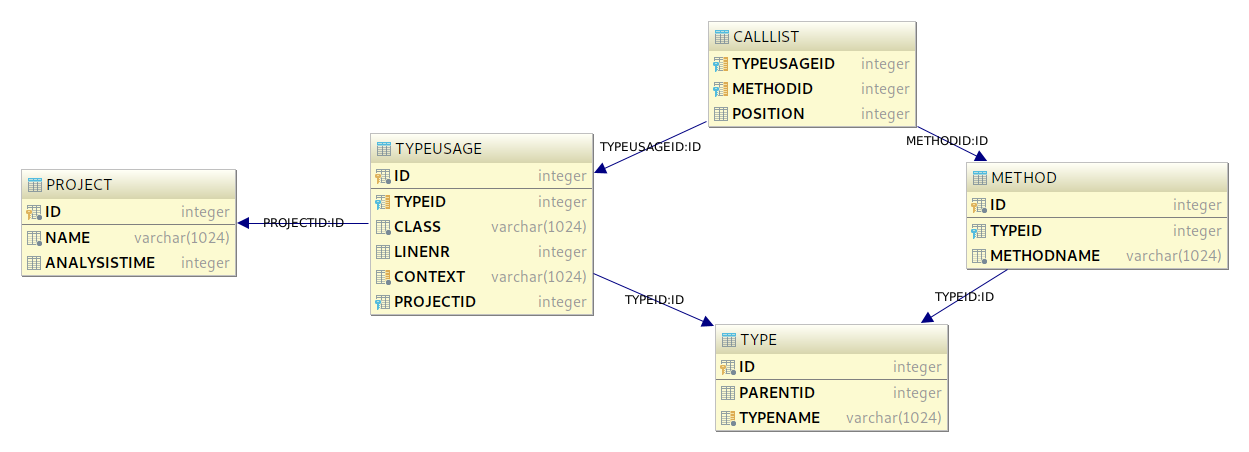
\includegraphics[width=\textwidth]{figures/database_layout-light}
    \caption{Overview of Database Tables}
    \label{fig:db_layout}
\end{figure}

%-- explain database layout 
Figure~\ref{fig:db_layout} depicts the layout of our database.
The central piece is the \code{TYPEUSAGE} table whose rows store the information related to one particular type usage.
This includes the class (complete with fully qualified package name) and the context in which the type usage occurred and, if possible, the line of code in which the object was first encountered.
Additionally, it references two other tables, \code{PROJECT} and \code{TYPE}.
In our setup, the \code{PROJECT} table describes the Android application from which the type usage was extracted together with the time it took to analyze this application.

The \code{TYPE} reference specifies to which type the type usage belongs.
Each type holds a reference to its parent type (if one exists), to enable rebuilding the inheritance hierarchy if so desired.
The methods that can be invoked on a type are stored in the \code{METHOD} table.
Finally, the \code{CALLLIST} table connects type usages and method calls and specifies which of the methods that \emph{could} be invoked are actually called on the type usage in question.

\section{Improvements and Dead Ends}\label{sec:deadends}

% general plan: explaining all the work i did + what was already there + why some solutions where discarded

% there exists code from monperrus et al., I took it and improved it
Monperrus et al.\ released their code and data on GitHub\footnote{\url{https://github.com/stg-tud/typeusage}}.
We started with their implementation and refactored it extensively\footnote{\url{https://github.com/ke-kx/typeusage}} to understand it better and to facilitate slight improvements like the database backend connection.
During the refactoring process, we discovered small discrepancies between what they describe in the paper and how their code behaves.
In the calculation of almost similarity between two type usages $x$ and $y$, the code only checks that the size of $M(y) \setminus M(x)$ is equal to one; however, it fails to verify that $M(x)$ does not include any other methods.
As such, in the situation that $M(x) =\{A, B, C\}$ and $M(y) = \{A, B, Z\}$, the code considers $y$ to be almost similar to $x$, because $y$ calls the additional method $Z$.
Recall that almost similarity expects one type usage to have one method call more than the other, and this is clearly not the case here with both type usages calling three methods.
However, we reran their experiments after correcting this small inaccuracy, and the results did not change significantly.

% attempt purely db solution -> db too slow
After we refactored the code and added the database backend, the database stores all of the type usage data.
Therefore, we thought it would be convenient to calculate the strangeness scores in the database as well and only query it for the finished results.
In hindsight, this was not the best idea.
The first query we designed to calculate the strangeness score was quite complicated, with many joins over views containing many more joins.
Even on a small test dataset, it was quite slow.
We attempted many improvements to the query, including better indices and smart cached subtables, but the query remained slow and memory intensive.
We even invested some time into exploring the possibility of using PostgreSQL\footnote{\url{https://www.postgresql.org/}}, but the results were equally disappointing.

% Better problem description + way to solution
Careful analysis revealed that the biggest problem was the one-by-one comparison of each type usage with all other type usages to determine their [almost / exact] similarity, resulting in runtime in $O(n^2)$ for $n$ type usages.
It seemed that the database was not able to unravel these numerous comparisons with our insufficient instruction.
However, if one thinks carefully about the process of determining the exact and almost similar type usages, something stands out: it is not necessary to compare all of the type usages one by one.
The only type usages that are potential candidates for exact or almost similarity are those that have the same type and context as the type usage under investigation.
%%however thinking about what happens - for each tu go through all tus, first check if type and context are the same (/only type for dmmc noContext) - only if that's the case go and compare the methods
This gives rise to natural partitions of the dataset: the sets of type usages which share the same type and context (or just the same type for the variant $\text{DMMC}_\text{noContext}$).
Within these partitions, we need to compare each type usage with all of the others, but each partition will only be a fraction of the size of the whole dataset.
Fortunately, the database is already perfectly suited for obtaining these subsets.
With this realization, we can continue to the final step of the analysis: detecting anomalies.

\section{Anomaly Detection}\label{sec:anomaly}

% overview of process

\todo[inline]{not super happy with this paragraph, but how to change it?}
% partitions + analysis
Some relatively simple Python scripts handle the anomaly detection.
The first step is to obtain the possible partitions of the dataset, depending on the variant, either all types in the dataset or all valid combinations of type and context.
\todo[inline]{This sentence was a bit confusing to me. I would change it to something like: "The first step is to partition the type usages by type for DMMCnoContext or a combination of type and context for DMMC. Obtaining these partitions is realized in the outer loop of the script with a simple query to the database: we iterate through all partitions and retrieve..."}
Observe that the database makes it very simple to obtain these partitions with just one query.
\todo{remove sentence?}
In its outer loop, the script iterates through all partitions and retrieves the type usages belonging to the current partition.
\todo[inline]{where do the partitions we iterate through come from? do we know them in advance? are they initialized beforehand or while iterating? it's a bit strange that we iterate through something we are just creating. maybe describe the outer loop a bit more detailed.}
Again, querying the database for these type usages is simple and also quite fast because of indices on the relevant columns.
% analysis
In the inner loop, the script iterates through all the type usages in the current partition and compares the methods that they invoke.
We compare each type usage with each other type usage only once, similar to filling an upper triangle matrix, thus saving nearly half of the comparisons.
% tear down / result
After determining the number of exactly and almost similar neighbors for each type usage in this manner, it is easy to calculate the strangeness score for all of them.
Finally, the script saves the results for further analysis and evaluation by an expert.

% other variants: loading
The anomaly detection is the only part of the implementation that is affected by the different variants presented in Chapter~\ref{ch:dmmc}.
We already mentioned the differences between including or excluding the context.
For the class merge variant, we perform some simple preprocessing before starting the analysis.
We load the data with type partitioning and merge those type usages which originated in the same class.
% other variants: anomalies
For the detection of superfluous or wrong method calls, we can use the same setup and only need to adapt the almost equal check to the new requirements.

